
\let\bold\bfseries
\let\italics\itshape
\def\Sum\mathlarger{\mathlarger{\sum}}

\subsection*{Time-Series Convolution%
  \label{time-series_convolution}%
  \addcontentsline{toc}{subsection}{Time Series Convolution}
}

\noindent  In these applications, $f$ is a waveform time series that is convolved with a pulse $g$.  The equation for the their convolution is
\begin{equation}
y(t) = f(t)\star g(t) \equiv \int_{-\infty}^\infty dt'\,f(t')g(t - t').
\end{equation}
Both $f$ and $g$ are functions of time, and their zero times are coupled through the term $g(t-t')$.  From Equation (1), it is easy to show that one can choose the time zero for $y$ and $f$ to be the same.  In the applications discussed below, the zero time for $g(t)$ can be the same as or less than the zero time for $f(t)$.
   
To calculate the convolution, one discretizes both $f$ and $g$ and replaces the integral with a sum.  In this discussion $\delta t = 0.02\,s$ is the digitizing interval for $y$, $f$, and $g$.  One multiplies the sum by $\delta t$, which is not what is done in a ``discrete convolution'', which also does not take into account any difference in zero time between $f(t)$ and $g(t)$.

In this document, two applications of convolution are discussed.  Both have the same $f(t)$ but different $g(t)$. 
\begin{itemize}
\item $f(t)$ is a synthetic waveform (produced using Haskell matrices or WKBJ) where vertical lines of calculated polarities and amplitudes are drawn at phase-arrival times.  For these examples, the synthetic waveform is a vertical-component time series for an incident $P$-wave at an angle of 20$^\circ$ with the vertical through a 2-layer crust. There are $n_w = 2048$ points in the discretized $f$.  (The large number is chosen to minimize wraparound.) The duration is $t_w = \delta t \,[n_w-1]$.  The first point in $f$ is chosen to be at $t = 0$, so $f(t) = f(t)\,H(t)\,H(t_w-t)$, where 
$$H(t) = \cases{1, &if $t > 0$;\cr 0,&if $t < 0$.\cr}.$$ 
 
\item $g(t)$ is a pulse waveform with a far smaller duration than $f(t)$.  Here, the pulse is either (1) an approximation of a $P$ arrival so that the output of the convolution potentially models the data, or (2) a time-symmetric shape with a maximum at $t=0$ to smooth out the Gibbs phenomenon that often accompanies arrivals in synthetics.  Option (2) is often used for synthetics for receiver functions.
  
A ``Brune'' pulse for (1): $g(t) = U_0\,H(t)t e^{- \frac{t}{\kappa}}\,H(t_p - t)$, where $\kappa = 0.1\,s$, $t_p = 1.26\,s$, and $U_0$ is a constant that only affects the amplitude, so is of no interest here. 

For (2), the source pulse is a triangle function produced by fg in SAC: 
\begin{quote}
fg triangle npts 8 delta 0.02 begin -0.08.
\end{quote}

Note that the Brune pulse starts at the same time as $f$, while the triangle pulse starts at a negative time with a maximum at the start time for $f$.  If the total time for the pulse is $t_p$, the general form for the pulse is $g(t) = g(t)\,H(t - t_1)\,H(t_2 - t)$, where for the Brune pulse $t_1 = 0, \ \ t_2 = t_p$ and for the triangle pulse $t_1 = -0.08\,s \ \ t_2 = 0.06\,s = t_p - t_1$.  For either pulse, $t_p = \delta t\,[n_p - 1]$.
\end{itemize}

Given the above forms for $f$ and $g$, Equation (1) can be written

\begin{equation}
y(t) = \int_0^{t_w} dt'\,f(t')g(t - t')\,H(t-t'-t_1)\,H(t_2-t+t').
\end{equation}
For the Brune pulse, $t_1 = 0$, so $t$ cannot be negative, but for the triangle pulse the lower bound for $t$ is -0.06\,s.   In Fortran, arrays are stored in the computer using positive integers, so to simplify the bookkeeping it is best to avoid negative times when we discretize Equation (2).   One can avoid negative times if one chooses $y(\tau) = y(t-t_1)$.  With this choice, Equation (2) then reads
\begin{equation}
y(\tau) = y(t-t_1) = \int_0^{t_w} dt'\,f(t')g(\tau+t_1 - t')\,H(\tau-t')\,H(t_2-\tau - t_1+t').
\end{equation}

The discretized equation for Equation (3) is 
\begin{equation}
y_i = \delta t \, \mathlarger{\mathlarger{\sum}}_{j=1}^{n_w}f_{j}\,g_{i-j-j_1}, 
\end{equation}
where $j_1 = -[t_1/\delta t]+1$ and $i$ runs from 1 to $n_w + n_p - 1$.


The following Fortran code produces the correct result for the convolution for either pulse:

\begin{verbatim}
        j_1 = -nint(b_p/delta)+1
        do i=1,n_w+n_p-1
          temp = 0.0
          do j=1,n_w
            if (i.ge.(j-j_1) .and. n_p.ge.(i-j+j_1))
     1          temp = temp + waveform(j)*pulse(i-j+j_1)
          end do
          conv(i) = delta*temp
        end do
\end{verbatim}
where b\_p = $t_1$, delta = $\delta t$, and conv(i) = $y_i$.

Plots for the two pulse waveforms are shown in Figure 1, and the results of the convolution near the first synthetic arrival are shown in Figure 2 both for the Brune pulse and for the triangle pulse. The Gibbs phenomenon is quite pronounced at the arrival in the raw synthetic.  Note that the peaks for the arrival in Figure 2 are at the same time for the triangle-pulse convolution and the synthetic, and the Brune-pulse convolution starts at the peak of the raw-synthetic arrival time. For display purposes, the waveforms are  time-shifted so that the first arrival are at five seconds into the record.  Hence the zero time for the display and the convolution calculation are not the same.

If one uses the SAC convolution for the two runs, one gets the ``correct'' result for the Brune pulse but a time shift of 0.08 seconds for the triangle pulse (which starts at -0.08\,s).  The convolution of the triangle pulse with itself is also time-shifted 0.08\,s.  If one uses the SAC CONVOLVE option ``amplitude on'' in program {\italics convolvef} or {\italics convovlec}, one gets the same amplitudes and times as for SAC convolution output.

\begin{figure}[ht]

\vspace{-0.5in}

\begin{center} \
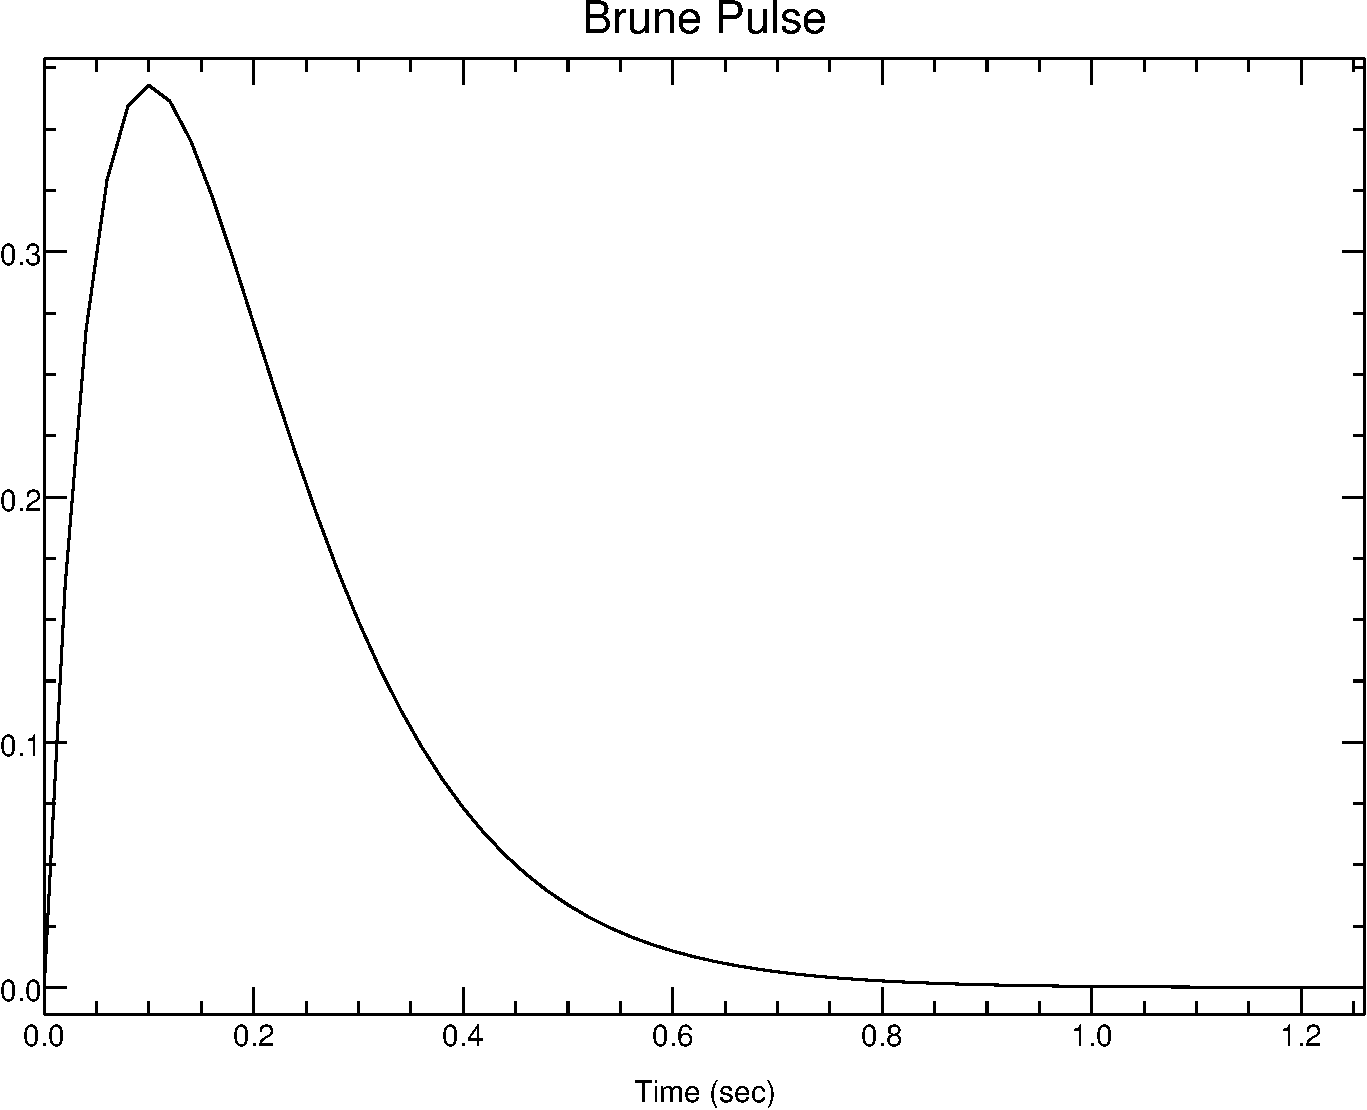
\includegraphics[width=0.45\textwidth]{./supplement/brune-pulse.pdf}
\hspace{0.1in}
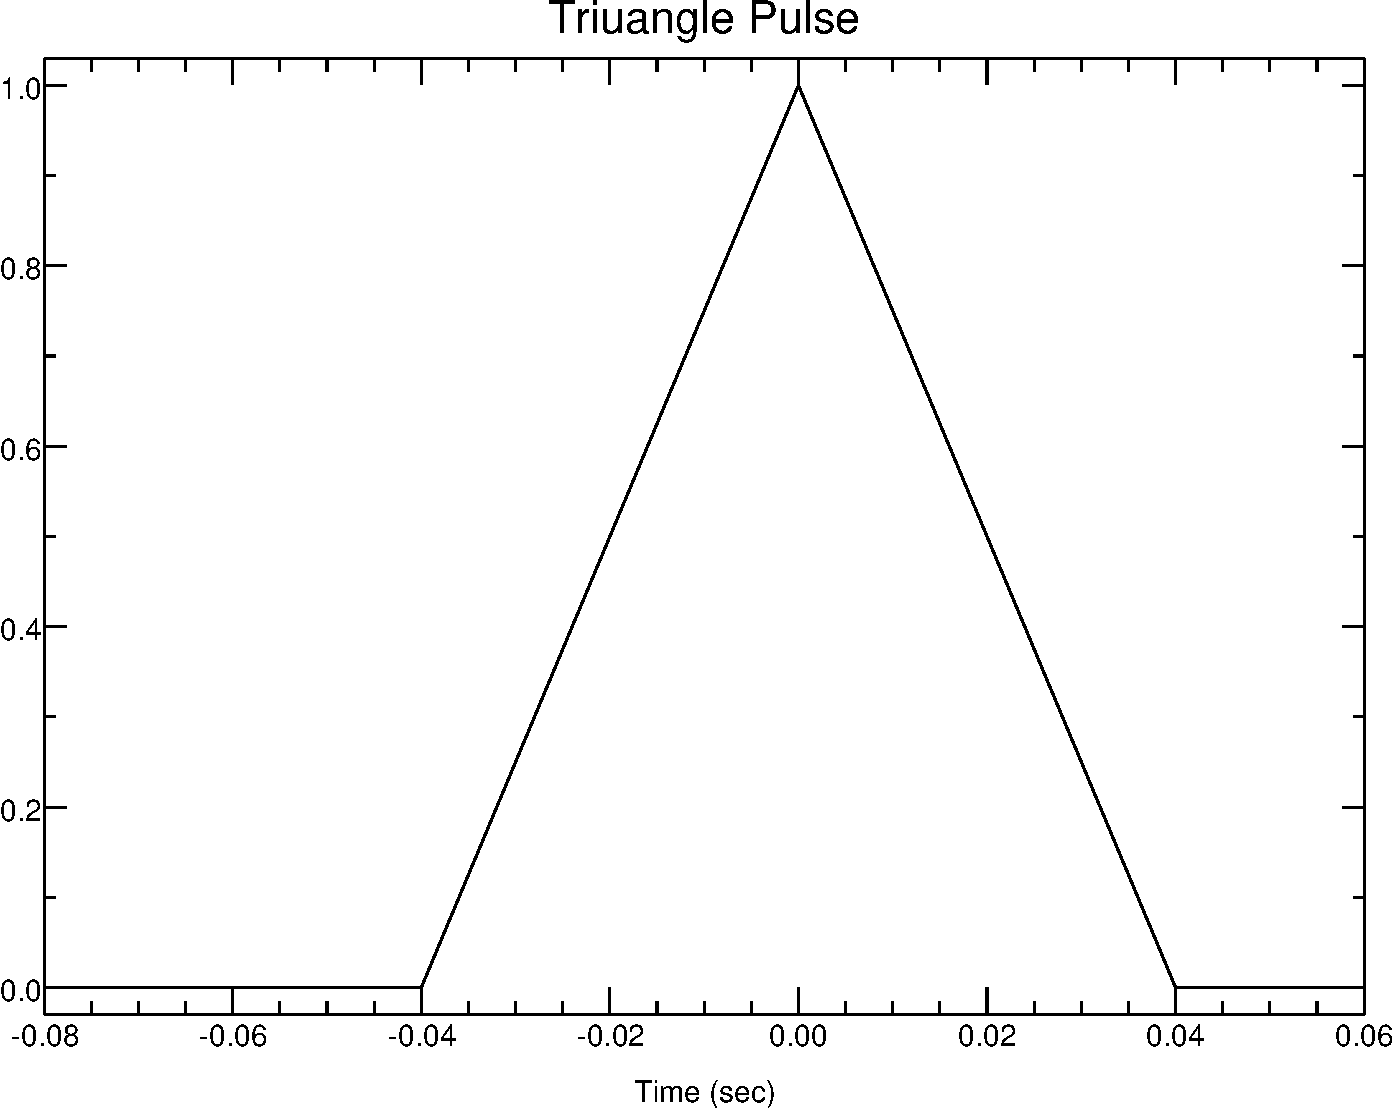
\includegraphics[width=0.45\textwidth]{./supplement/triangle-pulse.pdf}
\end{center} 

Figure 1: The two source pulses used for these convolution applications.

\vspace{-0.5in}

\begin{center} \
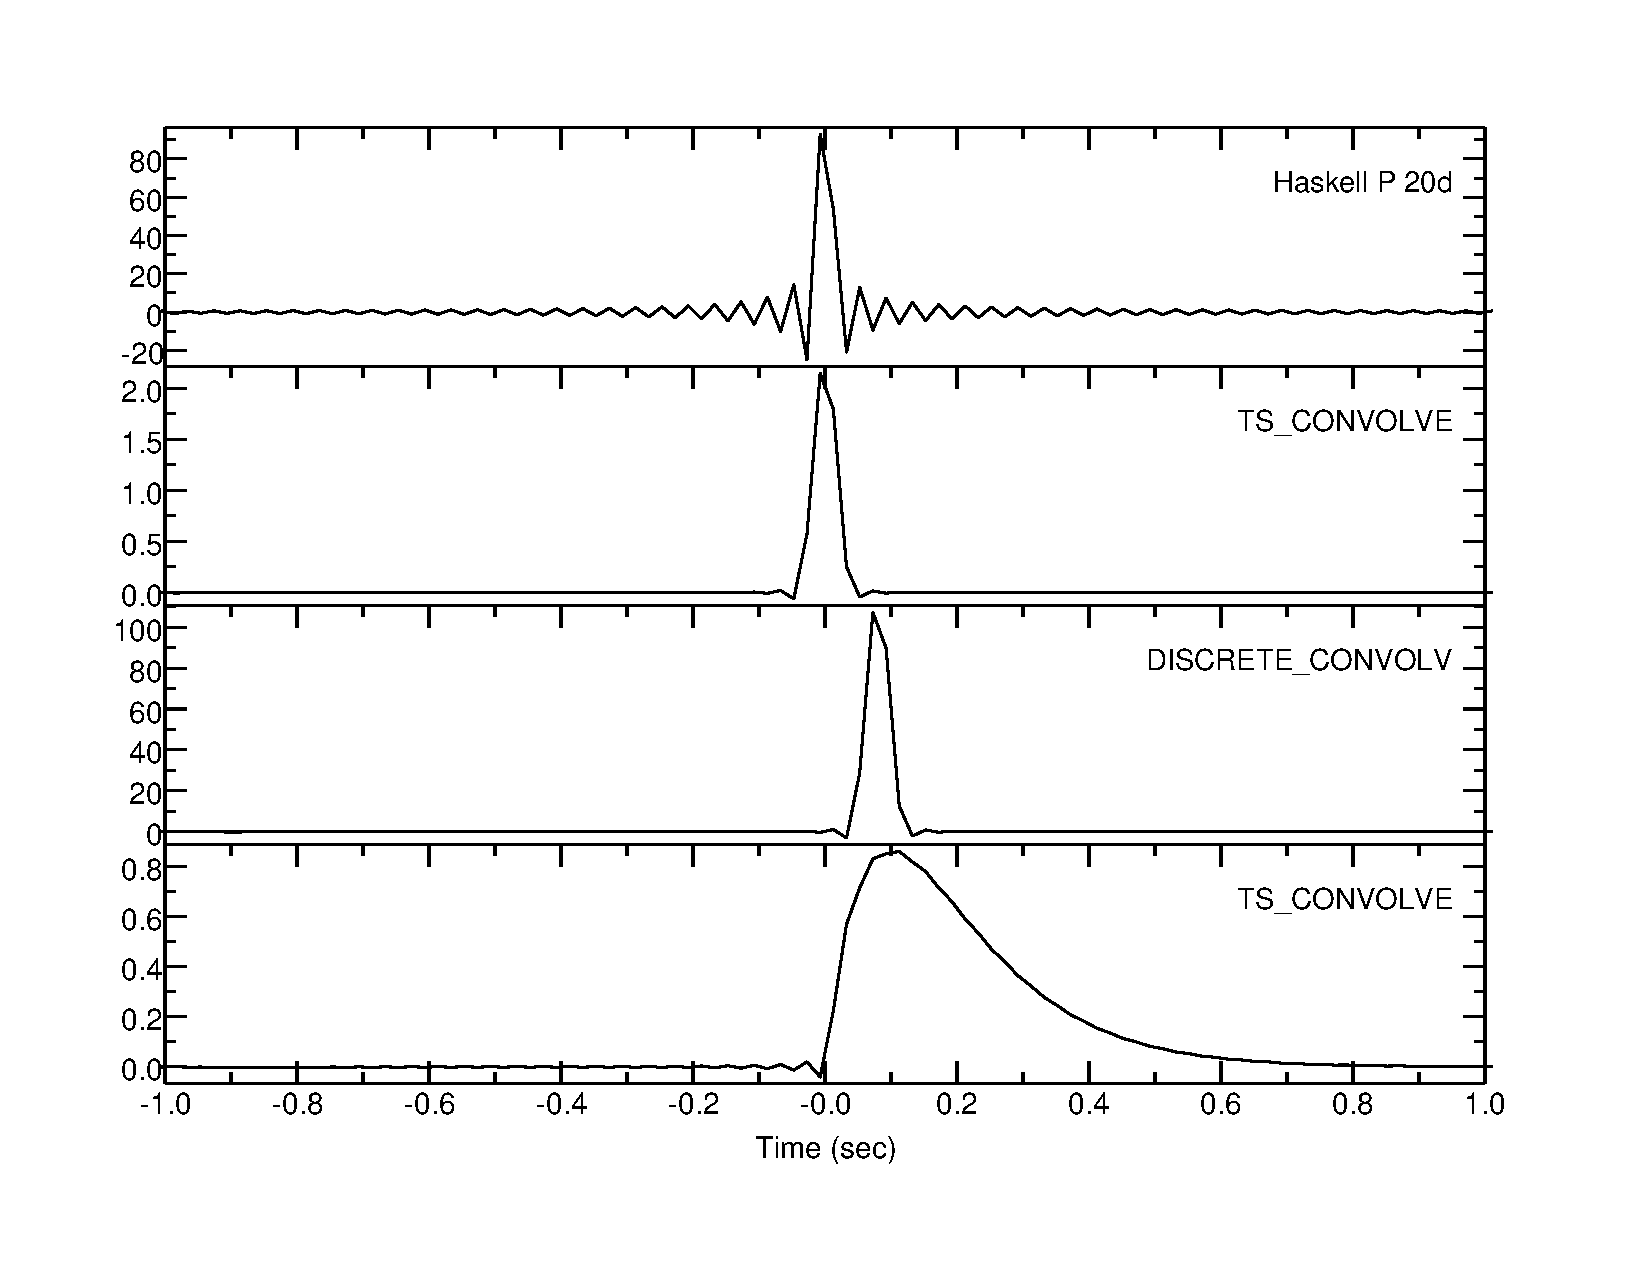
\includegraphics[width=0.95\textwidth]{./supplement/conv_pulse-synth.pdf}
\end{center} 

\vspace{-0.5in}

Figure 2: From top to bottom: unfiltered synthetic, time-series convolution with triangle pulse, discrete convolution with triangle pulse, time-series convolution with Brune pulse.
\end{figure}
